\documentclass[border=10pt,multi,tikz]{standalone}
\usepackage[edges]{forest}
\usetikzlibrary{arrows.meta, positioning}% arrows is deprecated
\usepackage{amssymb}
\usepackage[none]{hyphenat} % no hyphenation

\begin{document}
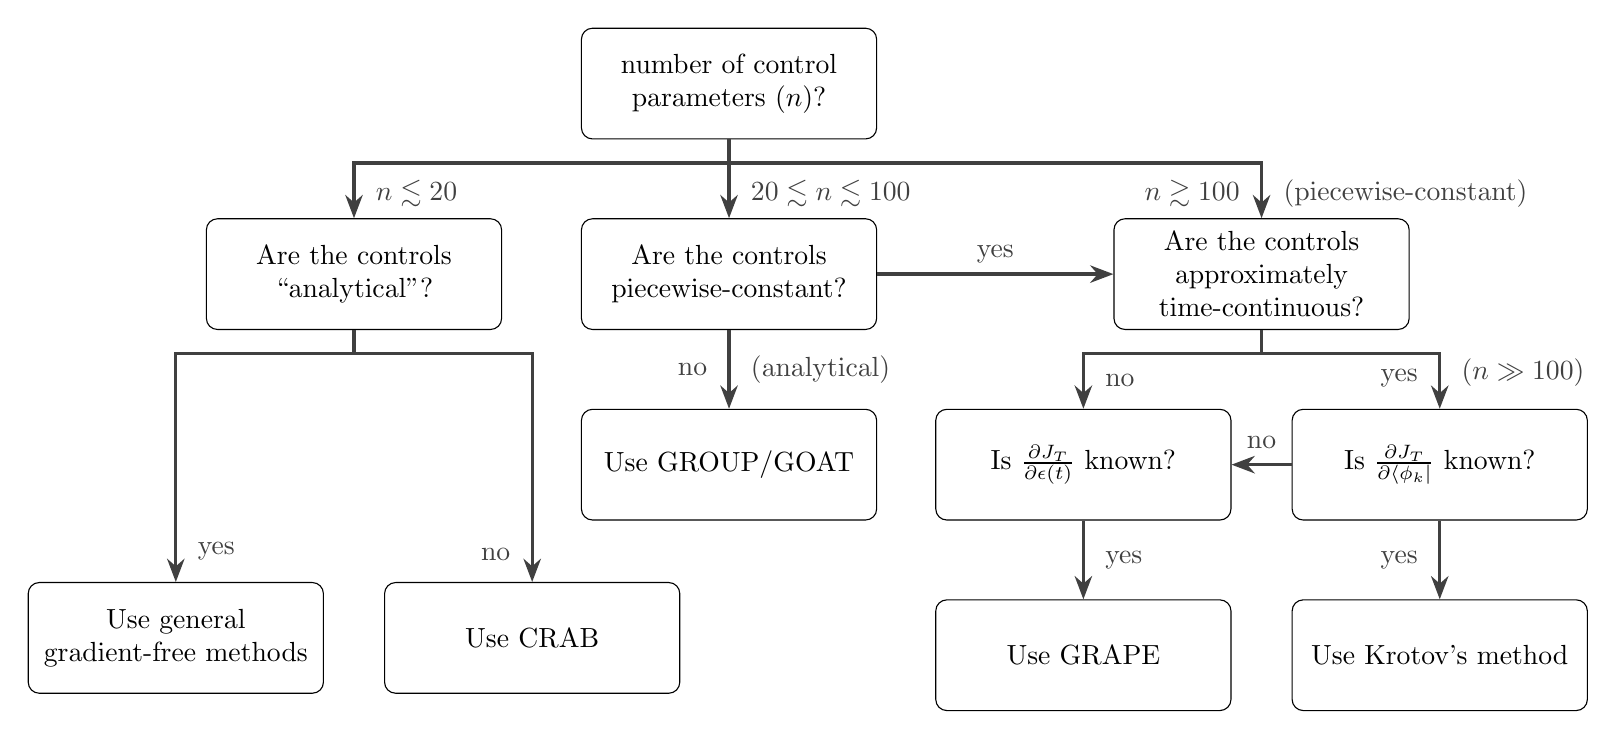
\begin{tikzpicture}[]
\tikzset{% \tikzstyle is deprecated
  block/.style={rectangle, draw, fill=white!20, text width=10em, text centered, rounded corners, minimum height=4em},
  line/.style={draw, very thick, color=black!75, -Stealth},
}
\newlength{\VertSep}
\setlength{\VertSep}{1cm}

\node[block] (NumberOfParameters) {number of control parameters ($n$)?};
\node[block, below left=\VertSep and 1cm of NumberOfParameters]
  (Analytical) {Are the controls ``analytical''?};
  \node[block, below left=3.2*\the\VertSep and -1.5cm of Analytical]
    (GradientFree) {Use general gradient-free methods};
  \node[block, below right=3.2*\the\VertSep and -1.5cm of Analytical]
    (CRAB) {Use CRAB};

\node[block, below=\VertSep of NumberOfParameters]
  (PWC) {Are the controls piecewise-constant?};
  \node[block, below=\VertSep of PWC]
    (UseGOAT) {Use GROUP/GOAT};

\node[block, below right=\VertSep and 3cm of NumberOfParameters]
  (Continuous) {Are the controls approximately time-continuous?};
  \node[block, below left=\VertSep and -1.5cm of Continuous]
    (GradientKnown){Is  $\frac{\partial J_T}{\partial \epsilon(t)}$ known?};
    \node[block, below=\VertSep of GradientKnown]
      (UseGRAPE) {Use GRAPE};
  \node[block, below right=\VertSep and -1.5cm of Continuous]
    (ChiKnown){Is $\frac{\partial J_T}{\partial \langle \phi_k\vert}$ known?};
    \node[block, below=\VertSep of ChiKnown]
      (UseKrotov){Use Krotov's method};

\draw[line] (NumberOfParameters.south) -- ++(0, -0.3*\the\VertSep)
  -| (Analytical.north)
  node[above right=0pt and 4pt] {$n \lesssim 20$};
\draw[line] (Analytical.south) -- ++(0, -0.3*\the\VertSep)
  -| (GradientFree.north)
  node[above right=4pt and 4pt] {yes};
\draw[line] (Analytical.south) -- ++(0, -0.3*\the\VertSep)
  -| (CRAB.north)
  node[above left=4pt and 4pt] {no};
\draw[line] (NumberOfParameters.south) -- ++(0, -0.3*\the\VertSep)
  -| (PWC.north)
  node[above right=0pt and 4pt] {$20 \lesssim n \lesssim 100$};
\draw[line] (PWC.south) -- (UseGOAT.north)
  node[midway, left=4pt] {no}
  node[midway, right=4pt] {(analytical)};
\draw[line] (PWC.east) -- (Continuous.west)
  node[midway, above] {yes};
\draw[line] (NumberOfParameters.south) -- ++(0, -0.3*\the\VertSep)
  -| (Continuous.north)
  node[above left=0pt and 4pt] {$n \gtrsim 100$}
  node[above right=0pt and 4pt] {(piecewise-constant)};
\draw[line] (Continuous.south) -- ++(0, -0.3*\the\VertSep)
  -| (GradientKnown.north)
  node[above right=4pt and 4pt] {no};
\draw[line] (Continuous.south) -- ++(0, -0.3*\the\VertSep)
  -| (ChiKnown.north)
  node[above left=4pt and 4pt] {yes}
  node[above right=4pt and 4pt] {($n \gg 100$)};
\draw[line] (GradientKnown.south) -- (UseGRAPE.north)
  node[midway, right=4pt] {yes};
\draw[line] (ChiKnown.south) -- (UseKrotov.north)
  node[midway, left=4pt] {yes};
\draw[line] (ChiKnown.west) -- (GradientKnown.east)
  node[midway, above=2pt] {no};
\end{tikzpicture}
\end{document}
